\documentclass[a4, 10pt]{article}


% +-----------------------------------------------------------------------------
% | Packages
% +-----------------------------------------------------------------------------

% AMS math packages
\usepackage{amsmath,amssymb}
\allowdisplaybreaks

% Proper unit placement
\usepackage{siunitx}

% Figure related packages
\usepackage{graphicx}
\usepackage[font={footnotesize}]{subfig}
\usepackage{placeins}

% Better tables
\usepackage{booktabs}

% Reference styling
\usepackage[noconfig]{refstyle}
%%--- TEMPLATE FOR FUNCs -------------------------
   \newref{func}{%
      name    = {Function~},
      names   = {Functions~},
      Name    = {Function~},
      Names   = {Functions~},
      rngtxt  = {\space to~},
      lsttxt  = {\space and~}}
%%--- TEMPLATE FOR ALGOS -------------------------
   \newref{algo}{%
      name    = {Algorithm~},
      names   = {Algorithms~},
      Name    = {Algorithm~},
      Names   = {Algorithms~},
      rngtxt  = {\space to~},
      lsttxt  = {\space and~}}
%%--- TEMPLATE FOR PARTS -------------------------
   \newref{part}{%
      name    = {Part~},
      names   = {Parts~},
      Name    = {Part~},
      Names   = {Parts~},
      rngtxt  = {\space to~},
      lsttxt  = {\space and~}}
%%--- TEMPLATE FOR CHAPTERS & APPENDIXES --------
   \makeatletter
   \providecommand*{\p@chapter}{}
   \renewcommand*{\p@chapter}{\string\chpname{\@chapapp}}
   \makeatother
   \newcommand*{\chpname}[1]{}
\newcommand*{\RSchpname}[1]{%
   \ifRSnameon%
      \edef\RStmpa{#1}%
      \edef\RStmpb{\appendixname}%
      \ifx\RStmpa\RStmpb\relax%
         \ifRSplural\ifRScapname{}Appendices~\else{}appendices~\fi
         \else\ifRScapname{}Appendix~\else{}appendix~\fi
         \fi
      \else%
         \ifRSplural\ifRScapname{}Chapters~\else{}Chapters~\fi
         \else\ifRScapname{}Chapter~\else{}Chapter~\fi
         \fi
      \fi
   \fi}
   \newref{chap}{%
      refcmd  = {\let\chpname=\RSchpname\ref{#1}},
      rngtxt  = {\space to~},
      lsttxt  = {\space and~}}
%%--- TEMPLATE FOR SECTIONS ---------------------
   \newref{sec}{%
      name    = {Section~},
      names   = {Sections~},
      Name    = {Section~},
      Names   = {Sections~},
      refcmd  = {\ref{#1}}, % was: \S\ref{#1}
      rngtxt  = {\space to~},
      lsttxt  = {\space and~}}
%%--- TEMPLATE FOR EQUATIONS --------------------
   \let\eqref\relax
   \newref{eq}{%
      name      = {Eq.~},
      names     = {Equations~},
      Name      = {Equation~},
      Names     = {Equations~},
      refcmd    = \textup{(\ref{#1})},
      rngtxt    = {\space to~},
      lsttxt    = {\space and~}}%
%%--- TEMPLATE FOR FIGURES ----------------------
   \newref{fig}{%
      name    = {Figure~},
      names   = {Figures~},
      Name    = {Figure~},
      Names   = {Figures~},
      rngtxt  = {\space to~},
      lsttxt  = {\space and~}}
%%--- TEMPLATE FOR TABLES -----------------------
   \newref{tab}{%
      name    = {Table~},
      names   = {Tables~},
      Name    = {Table~},
      Names   = {Tables~},
      rngtxt  = {\space to~},
      lsttxt  = {\space and~}}
%%--- TEMPLATE FOR FOOTNOTES --------------------
   \makeatletter
   \newcommand{\RSfnmark}[1]{%
      \begingroup
        \unrestored@protected@xdef\@thefnmark{#1}%
      \endgroup
      \@footnotemark}
   \makeatother
   \newref{fn}{%
      name    = {Footnote~},
      names   = {Footnotes~},
      Name    = {Footnote~},
      Names   = {Footnotes~},
      refcmd  = {\ifRSstar\RSfnmark{\ref{#1}}\else\ref{#1}\fi},
      rngtxt  = {\space to~},
      lsttxt  = {\space and~}}
%%--- TEMPLATE FOR THEOREMS ---------------------
   \newref{thm}{%
      name    = {Theorem~},
      names   = {Theorems~},
      Name    = {Theorem~},
      Names   = {Theorems~},
      refcmd  = {\ref{#1}}, % was: \S\ref{#1}
      rngtxt  = {\space to~},
      lsttxt  = {\space and~}}
%%--- TEMPLATE FOR DEFINITIONS ---------------------
   \newref{def}{%
      name    = {Definition~},
      names   = {Definitions~},
      Name    = {Definition~},
      Names   = {Definitions~},
      refcmd  = {\ref{#1}}, % was: \S\ref{#1}
      rngtxt  = {\space to~},
      lsttxt  = {\space and~}}
\endinput
%%
%% End of file `reftmpl.cfg'.


% Source code formatting
\usepackage{minted}
\usemintedstyle{friendly}
 
% Tikz setup
\usepackage{tikz}
\usetikzlibrary{external}
%\tikzexternalize[prefix=tikz/]
% Define good colors
\definecolor{col1}{rgb}{1.00, 0.14, 0.14}
\definecolor{col2}{rgb}{0.13, 0.17, 0.53}
\definecolor{col3}{rgb}{0.99, 0.68, 0.38}
\definecolor{col4}{rgb}{0.67, 0.87, 0.64}

\definecolor{linkcol}{rgb}{0.039, 0.336, 0.527}

% Fixme notes
\usepackage{fixme}
\fxsetup{%
    status=draft,
    theme=color
}

% Comment boxes
\usepackage[tikz]{bclogo}

% Hyperref configuration
\usepackage{hyperref}
\hypersetup{
    colorlinks=true,
    linkcolor=linkcol,
    urlcolor=linkcol,
    % PDF attributes
    pdfauthor={Lionel Ott},
    pdftitle={Joystick Gremlin Manual},
}

% Citation format
\usepackage[square,numbers,comma,sort]{natbib}

% Redefine the \vec command to use bold font instead of an arrow
\DeclareMathOperator*{\argmax}{\arg\!\max}

% Text replacement commands
\newcommand{\JG}{Joystick Gremlin}


\begin{document}

\begin{titlepage}
\begin{center}
	\vspace*{\fill}
	\vspace*{-3cm}
    \begin{Huge}
        \textbf{Joystick Gremlin}
    \end{Huge}

    \vspace{1cm}

    \begin{Large}
        {Manual for Release 2}
    \end{Large}

    \vspace{3cm}

    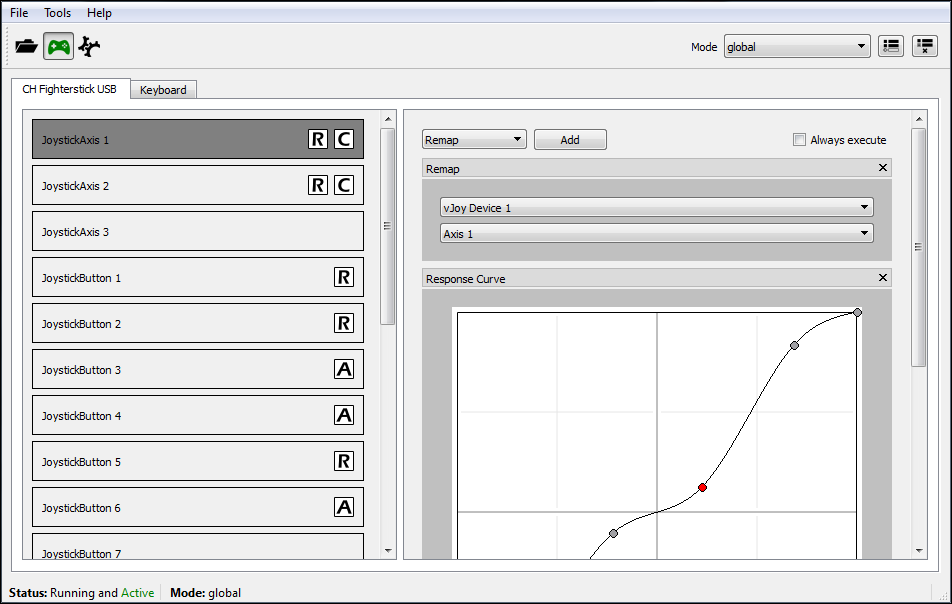
\includegraphics[width=0.9\linewidth]{images/main_screen}

    \vspace{6.0cm}

	March 2015
\vspace*{\fill}
\end{center}
\end{titlepage}


\tableofcontents
\newpage


% +-----------------------------------------------------------------------------
% | Introduction
% +-----------------------------------------------------------------------------
\section{Introduction}
\label{sec:introduction}


\subsection{Overview}

\JG{} is a program that allows the configuration of joystick like
peripherals. It is similar to programs such as CH Products' CH Control
Manager and Thrusmaster's T.A.R.G.E.T. However, it is manufacturer
agnostic and thus works with devices from any manufacturer and uses
Python as its scripting. The major features of Joystick Gremlin are:
\begin{itemize}
    \item Merging of multiple devices into a single device
    \item Axis response curve and dead zone configuration
    \item Arbitrary number of modes with customisable mode switching
    \item Keyboard macros
    \item Python scripting support
\end{itemize}

\JG{} can be used via a graphical user interface or a simple console
script. The UI allows commonly performed tasks, such as input remapping,
axis response curve setups, and macro recording to be performed using a
graphical interface. Functionality that is not accessible via the UI can
be implemented through custom modules, see \secref{custom_modules}. The
console program uses these custom modules exclusively.


\subsection{Installation}
\JG{} has one major dependency, vJoy which provides virtual joysticks
which \JG{} feeds with data. Download links to the programs needed are
listed below:
\begin{itemize}
    \item \href{https://github.com/WhiteMagic/JoystickGremlin}{\JG{}}
    \item \href{http://vjoystick.sourceforge.net/site/}{vJoy}
    \item
        \href{http://www.microsoft.com/en-us/download/details.aspx?id=5555}{VC
        Redistributable 2010}
\end{itemize}

vJoy creates virtual joysticks which show up as a device in Windows and
\JG{} uses these to forward inputs to them. The VC2010 package is
required by Python but is likely to already be installed.

\subsubsection{vJoy Configuration}

In order to properly use \JG{} vJoy has to be configured first. This is
done via the \emph{Configure vJoy} program. This program allows setting
the properties of all existing vJoy devices. Typically a single vJoy
device is enough. In order to use 8-way POV hats with \JG{} the hats
have the be configured as continuous in vJoy. Once everything is set as
desired clicking \emph{Ok} configures the vJoy device and closes the
program.

\begin{figure}[bt]
    \centering

    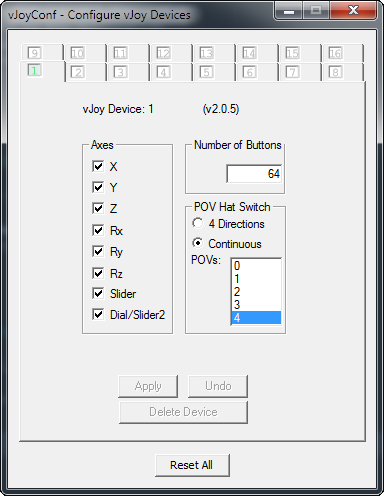
\includegraphics[width=0.5\linewidth]{images/vjoy_configuration}
    \caption{vJoy Configuration program showing the correct setting for
        the POV hats as well as having all 8 axis and 64 buttons
        configured.}
\end{figure}


\subsection{Concepts}
\label{sec:concepts}

The following section introduces the terminology used by \JG{}.


\subsubsection{Profile}
A profile is a folder which contains a XML configuration file together
with any custom modules used. The profile contains the settings made via
the user interface for each of the connected peripherals.

\subsubsection{Input}
An input is an axis, button, hat, or keyboard key on a physical device.
Each input can have multiple actions assigned to it and these actions
can change between the different modes.

\subsubsection{Action}
An action is something \JG{} executes when an input is used. Examples
are running a macro, sending button presses to vJoy, or changing to a
different mode. Each action has a condition attached to it which
dictates when it is executed. For buttons this is the state, i.e.\
pressed or released.

\subsubsection{Mode}
A mode is a collection of actions associated with the various inputs.
Each mode is independent of all other modes, i.e.\ their settings do
never conflict as only a single mode is active at any point in time.

An exception to this is the \emph{global} mode. This mode always exists
and allows for settings to be shared between all modes. However, global
actions will only be used if a mode has no actions associated with a
given input.



% +-----------------------------------------------------------------------------
% | Using the User Interface
% +-----------------------------------------------------------------------------
\section{Using the User Interface}
\label{sec:gui}

In the following the various components of the user interface are
introduced and their usage described. The UI should be sufficient for
most common use cases, however, if functionality is missing user created
modules can provide these.


\subsection{Overview}

The following is a short overview of the different components that make
up the main user interface, shown in \figref{main-ui}.

\begin{figure}[bt]
    \centering

    \begin{tikzpicture}[
        box/.style={
            draw=red,
        },
        label/.style={
            color=red,
        }
    ]
        \node [anchor=south west, inner sep=0] (image) at (0, 0)
            {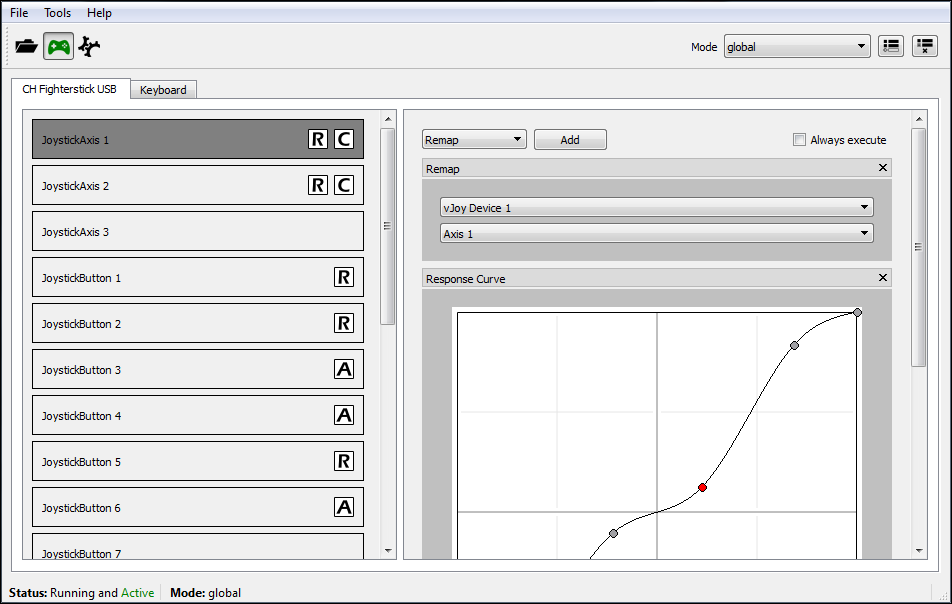
\includegraphics[width=0.95\linewidth]{images/main_screen}};

        \begin{scope}[x={(image.south east)},y={(image.north west)}]
            % Input item scroll list
            \draw [box] (0.02, 0.825) rectangle (0.42, 0.065);
            \node [label] at (0.20, 0.10) {1};

            % Input item configuration
            \draw [box] (0.43, 0.825) rectangle (0.98, 0.065);
            \node [label] at (0.70, 0.10) {2};

            % Mode selector / editor
            \draw [box] (0.72, 0.96) rectangle (0.99, 0.89);
            \node [label] at (0.70, 0.93) {3};

            % Status display
            \draw [box] (0.005, 0.04) rectangle (0.26, -0.005);
            \node [label] at (0.28, 0.02) {4};

            % Toolbar icons
            \draw [box] (0.01, 0.96) rectangle (0.12, 0.89);
            \node [label] at (0.14, 0.93) {5};

            % Device tabs
            \draw [box] (0.01, 0.87) rectangle (0.21, 0.83);
            \node [label] at (0.23, 0.85) {6};

            %\draw[help lines,xstep=.1,ystep=.1] (0,0) grid (1,1);
            %\foreach \x in {0,1,...,9} { \node [anchor=north] at (\x/10,0) {0.\x}; }
            %\foreach \y in {0,1,...,9} { \node [anchor=east] at (0,\y/10) {0.\y}; }
        \end{scope}
    \end{tikzpicture}

    \caption{The main screen of the user interface.}
    \label{fig:main-ui}
\end{figure}

\begin{enumerate}
    \item Overview of all the inputs available for a given device. The
        small icons on the far right of each input indicate the type of
        actions associated with the input. \emph{A} is a control action,
        \emph{C} is a response curve, \emph{M} is a macro, and \emph{R} is
        a remapping.
    \item The right hand portion of the UI shows the list of actions
        associated with the currently selected input. This panel allows
        the customisation of existing actions and the addition of new
        ones.
    \item The mode management section allows changing the mode currently
        being configured as well as adding and removing existing modes.
    \item The status bar shows whether or not the program is currently
        running a profile and if so the currently active mode is shown
        as well as whether or not code execution is paused.
    \item Tool bar with the main actions, from left to right
        \begin{itemize}
            \item Open an existing profile, discarding the current one
                and any unsaved changes to it.
            \item Activate \JG{}, when active the button is pressed and
                a green icon is shown. This also changes the status bar
                display. Pressing it again disables \JG{}.
            \item Generate code, this generates a configuration based on
                the current settings. This is also done automatically
                when \JG{} is activated.
        \end{itemize}
    \item Each tab represents an individual device that is currently
        connected to the computer.
\end{enumerate}


\subsection{Actions}

As described in \secref{concepts}, each input, such as axis, button,
hat, or keyboard key, can have multiple actions associated with them.
However, not all inputs have access to the same types of actions as they
are not applicable to them. The following section describes all the
available actions.

Each action has an activation condition associated with it which can be
used for fine grained control over them. Additionally, each input can
also be configured to be always executed by checking the box near the
\emph{Always Execute} text in the top right corner. If this is used then
the associated actions will be performed even if execution is paused.
This is mainly useful for resuming when execution has been pause.

\vspace{1em}
\begin{bclogo}[
    couleur=yellow!40,
    couleurBord=orange!80,
    couleurBarre=orange!80,
    arrondi=0.1,
    logo=\bcinfo
]{Note}
    Conditions are currently only implemented for joystick buttons and
    keyboard keys.
\end{bclogo}


\subsubsection{Remapping}

\begin{figure}[bt]
    \centering

    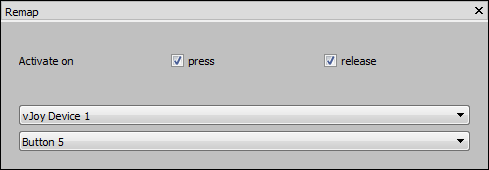
\includegraphics[width=0.75\linewidth]{images/action_remap}
    \caption{Remap widget allowing the mapping of a physical joystick
        input to an equivalent input on a vJoy device.}
    \label{fig:action_remap}
\end{figure}

The remapping action, shown in \figref{action_remap}, enables the user
to propagate inputs from a physical joystick input to an equivalent vJoy
input, i.e.\ axis to axis, button to button and hat to hat.  This for
example allows the merging of multiple physical devices into a single
device.

\vspace{1em}
\begin{bclogo}[
    couleur=yellow!40,
    couleurBord=orange!80,
    couleurBarre=orange!80,
    arrondi=0.1,
    logo=\bcinfo
]{Note}
    In most cases remap actions should always trigger, i.e.\ on button press and
    release, as otherwise the forwarding to vJoy is incomplete.
\end{bclogo}


\subsubsection{Response Curve}

\begin{figure}[bt]
    \centering

    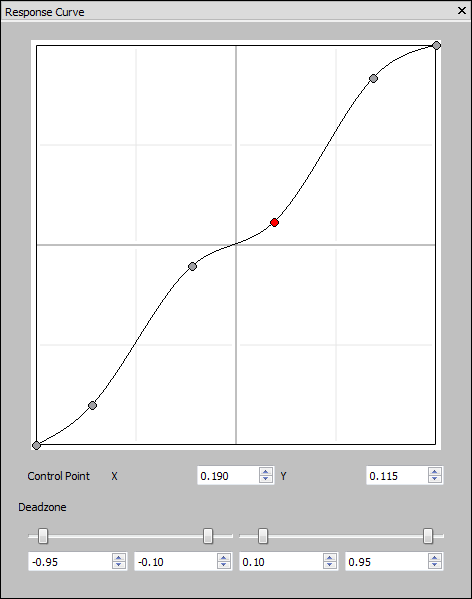
\includegraphics[width=0.75\linewidth]{images/action_response_curve}
    \caption{The response curve dialogue allows the customisation of the
        joystick response as well as the dead zone.}
    \label{fig:action_response_curve}
\end{figure}

The response curve dialogue, shown in \figref{action_response_curve},
allows the customisation of the response produced by the joystick using
the curve editor. The shape of the curve is controlled using a set of
control points which are used to define a cubic spline.

A new control point is added by a double left click in an empty area of
the curve editor. Removing an existing control point is achieved by a
double right click on the desired point. A single left click on a
control point will mark the point as active. An active point can be
dragged in the window to modify it's position. Alternatively, the text
fields below the curve editor allow for precise numerical values to be
entered.

Finally the dead zones for the axis can be defined using the sliders and
input fields at the bottom of the dialogue. The fields and sliders
control the full deflection dead zone, left and right inputs, as well as
the centre deflection dead zones, two centre inputs.

Currently there are two types of response curve types available:
\begin{description}
    \item[Cubic Spline] A simple spline with only control points dictating
        locations the curve has to pass through. No control over the
        shape is provided.
    \item[Cubic B\'{e}zier Spline] A more complex spline with control
        points and ``handles'' that can modify the shape of the overall
        curve. Importantly this curve allows the control of how the
        curve approaches the end points of the curve.
\end{description}

\begin{bclogo}[
    couleur=yellow!40,
    couleurBord=orange!80,
    couleurBarre=orange!80,
    arrondi=0.1,
    logo=\bcinfo
]{Note}
    A response curve mapping action always needs to be paired with a
    remap action, as otherwise the transformation will not have any
    effect.
\end{bclogo}

\vspace{1em}

\begin{bclogo}[
    couleur=yellow!40,
    couleurBord=orange!80,
    couleurBarre=orange!80,
    arrondi=0.1,
    logo=\bcinfo
]{Note}
    In order for response curves to work properly the game has to be
    configured to use a linear 1:1 curve, as otherwise the two curve
    settings will interfere with each other producing undesirable
    results.
\end{bclogo}


\subsubsection{Macro}

\begin{figure}[bt]
    \centering

    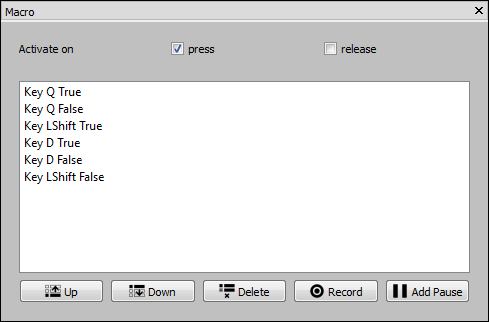
\includegraphics[width=0.75\linewidth]{images/action_macro}
    \caption{Macro recording widget containing a simple sequence of
    keys.}
    \label{fig:action_macro}
\end{figure}

The macro dialogue, see \figref{action_macro}, allows the creation of
keyboard macros. The macro can contain any combination of key presses
and releases, as well as pauses between individual actions.

Adding new keystrokes to a macro is done by pressing the \emph{Record}
button, after which all keystrokes will be recorded sequentially. To
stop the recording simply press the \emph{Record} button again. A pause
can be added by pressing the \emph{Add Pause} button, which will insert
a pause after the currently selected entry. The length of the pause can
be modified by double clicking the entry. Selecting an entry allows it
to be moved up and down using the \emph{Up} and \emph{Down} buttons.

\vspace{1em}
\begin{bclogo}[
    couleur=yellow!40,
    couleurBord=orange!80,
    couleurBarre=orange!80,
    arrondi=0.1,
    logo=\bcinfo
]{Note}
    Each macro is executed independently, which means that multiple long
    running macros can have their key presses interfere with each other.
\end{bclogo}


\subsubsection{Pause \& Resume}

\begin{figure}[bt]
    \centering

    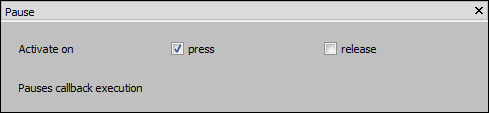
\includegraphics[width=0.75\linewidth]{images/action_pause}
    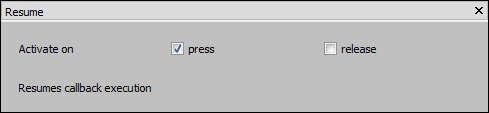
\includegraphics[width=0.75\linewidth]{images/action_resume}

    \caption{Pause and resume action dialogues.}
    \label{fig:action_pause_resume}
\end{figure}

The pause and resume actions, shown in \figref{action_pause_resume},
control whether or not \JG{} executes callbacks when inputs are used.
When the application is paused only inputs that were configured to
\emph{always trigger} will be executed.  The resume action instructs
\JG{} to process all inputs.

\vspace{1em}
\begin{bclogo}[
    couleur=yellow!40,
    couleurBord=orange!80,
    couleurBarre=orange!80,
    arrondi=0.1,
    logo=\bcinfo
]{Note}
    In order for the \emph{resume} action to be useful it has to be
    defined as \emph{Always Execute}, as otherwise it will be impossible
    to resume from the paused state.
\end{bclogo}


\subsubsection{Change Mode}

\begin{figure}[bt]
    \centering

    
\includegraphics[width=0.75\linewidth]{images/action_switch_mode}
    \caption{Change mode dialogue configured to switch to the
        \emph{hornet} mode.}
    \label{fig:action_change_mode}
\end{figure}

This action will change the currently active mode of \JG{} to the
specified one. The dialogue,  shown in \figref{action_change_mode}, has
a simple drop down list which contains all the available modes.


\subsubsection{Switch to Previous Mode}

\begin{figure}[bt]
    \centering

    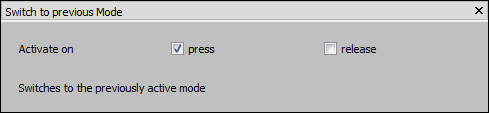
\includegraphics[width=0.75\linewidth]{images/action_switch_previous_mode}
    \caption{Dialogue of the action that switches to the previously
    active mode.}
    \label{fig:action_previous_mode}
\end{figure}

When the input with which this action, \figref{action_previous_mode}, is
activated the active mode of \JG{} will change to the previously active
one.


\subsubsection{Cycle Modes}

\begin{figure}[bt]
    \centering

    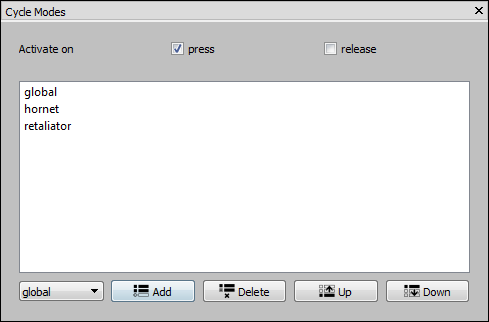
\includegraphics[width=0.75\linewidth]{images/action_cycle_modes}
    \caption{Mode cycling action dialogue which switches between the
        \emph{global}, \emph{hornet}, and \emph{retaliator} modes.}
    \label{fig:action_cycle_modes}
\end{figure}

This action, shown in \figref{action_cycle_modes}, allows the
configuration of a list of modes that are cycled through consecutively
with each activation. In case that the currently active mode is not part
of the list the first mode in the list will be activated.

New modes can be added by selecting the desired mode in the drop down
list and pressing the \emph{Add} button. The currently selected mode can
be deleted by pressing the \emph{Delete} button and moved up or down
with the \emph{Up} and \emph{Down} button respectively.

\FloatBarrier


\subsection{Tools}

In the following section the various tools provided by \JG{} are
described. They can be accessed via the \emph{Tools} menu in the menu
bar.

\subsubsection{Custom Module Management}

\begin{figure}[bt]
    \centering

    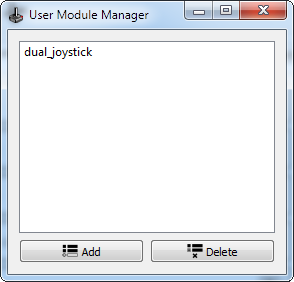
\includegraphics[width=0.3\linewidth]{images/module_manager}
    \caption{Module manager window loading a single external module.}
    \label{fig:custom_module}
\end{figure}

While the UI exposes commonly performed customisations there is
functionality that is not present. However, by using custom modules,
described in \secref{custom_modules}, the limitations of the UI can
easily be overcome. The module configuration dialogue,
\figref{custom_module}, can be opened via \emph{Tools $\rightarrow$
Manage Custom Modules}. The modules listed here will be loaded in
conjunction with the UI based configuration, allowing the use of the UI
for common tasks and implementing specialised functionality in a custom
module. Modules are added via the \emph{Add} button and likewise removed
by selecting the desired module and pressing the \emph{Delete} button.


\subsubsection{Device Information}

\begin{figure}[bt]
    \centering

    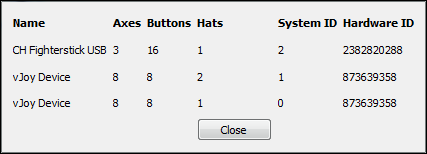
\includegraphics[width=0.75\linewidth]{images/device_information}
    \caption{Overview of the inputs and identification of the various
        joystick devices present in the system.}
    \label{fig:device_information}
\end{figure}

Information about connected devices can be accessed via \emph{Tools
$\rightarrow$ Device Information}. This window, shown in
\figref{device_information}, provides an overview of the devices known
to \JG{}, listing the name as well as some basic information of each
device. The \emph{System ID} represents the order in which the devices
are seen by the operating system, while the \emph{Hardware ID} is an
identifier that is unique to each device.

\vspace{1em}
\begin{bclogo}[
    couleur=yellow!40,
    couleurBord=orange!80,
    couleurBarre=orange!80,
    arrondi=0.1,
    logo=\bcinfo
]{Note}
    The currently used hardware id is not device, but product specific.
    As such it can not distinguish between two identical joysticks. To
    distinguish those the system id is used. When there are no duplicate
    devices present the system id is ignored.
\end{bclogo}


\subsubsection{Input Repeater}

By enabling the \emph{Input Repeater} option via \emph{Tools
$\rightarrow$ Input Repeater}, \JG{} will repeat the last remapped input
after a short wait period. This allows button presses and axes movements
to be mapped in-game when the game picks up the physical device over the
virtual one.


\subsubsection{Calibration}

The axes calibration screen can be accessed via \emph{Tools
$\rightarrow$ Calibration}. This screen allows the selection of the
device to calibrate. To calibrate the axes simply move them through
their full range and press the \emph{Center} button when all axes are
centered. Once done press \emph{Save} to save the calibration to the
configuration file.



% +-----------------------------------------------------------------------------
% | Using the Console Program
% +-----------------------------------------------------------------------------
\section{Using the Console Program}
\label{sec:console}

As mentioned there is also a command line version of \JG{}. This
version does not allow any configuration of settings but simply uses
user provided modules, covered in \secref{custom_modules}. This is
intended for users that wish to write completely customised
configurations making use of Python scripting without the UI ever being
shown.

An example usage of the console program is as follows:
\begin{minted}{bash}
    ./console_only profile_folder global hornet hull_c
\end{minted}

This starts the program and adds the folder \verb+profile_folder+ to
Python's module path and then loads the contents of the \verb+global+,
\verb+hornet+, and \verb+hull_c+ modules.


% +-----------------------------------------------------------------------------
% | Writing Custom Modules
% +-----------------------------------------------------------------------------
\section{Writing Custom Modules}
\label{sec:custom_modules}

While common configuration tasks can be performed directly via the UI,
more advanced and specialised configurations require writing custom
modules. Each module is a simple Python script which defines callbacks
triggered in reaction to inputs being used. Since the callbacks are
written in Python there is no limit to what can be expressed. In the
following \secref{cm_principles} provides a general overview of the
layout of a custom module, followed by an overview of the API in
\secref{cm_api}, before a few examples are shown in
\secref{cm_examples}.


\subsection{Principle \& Layout of Custom Modules}
\label{sec:cm_principles}

Joystick Gremlin uses callbacks, i.e.\ functions that are executed in
reaction to user inputs such as key presses or axis motions. These
callbacks have access to some convenience functions which allow
accessing and controlling often used parts of the system, such as
setting the value of vJoy devices or retrieving keyboard and joystick
states. Combining these readily available functions with custom code
allows the implementation of varied functionality.

The general structure of a callback is as follows:
\begin{minted}{python}
    @decorator_function(<input name>)
    def callback_function(event, <optional parameter list>):
        <callback implementation>
\end{minted}

The \verb+event+ parameter contains information about the event that
triggered the execution of the function. Each event is of type
\verb+gremlin.event_handler.Event+ and contains the following data:

\begin{itemize}
    \item \verb+event_type+, the type of the event, which is predetermined by
        the decorator function that was used to decorate the function
    \item \verb+identifier+, the identifier of the input, specified by the
        input name used in the decorator
    \item \verb+hardware_id+, the hardware id of the device, predetermined by the
        decorator function that was used to decorate the function
    \item \verb+windows_id+, the windows id of the device, predetermined by the
        decorator function that was used to decorate the function
    \item \verb+is_pressed+, indicates if a button or key is pressed or
        released, only valid for joystick buttons or keyboard keeys
    \item \verb+value+, value of an axis or hat, only valid fro joystick axes
        or hats
    \item \verb+raw_value+, the raw axis value, if the \verb+event_type+
        represents an axis
\end{itemize}

From this list the only values that are typically of interest are the
\verb+is_pressed+ and \verb+value+ entries.


\subsection{API}
\label{sec:cm_api}

The following describes the API of the variables exposed via the
decorator callback framework.


\subsubsection{vJoy}

Any decorated function that has a parameter named \verb+vjoy+ in its
parameter list will have access to all vJoy devices.  Accessing a
specific \verb+VJoy+ instance is done by indexing the \verb+vjoy+
object. This object then allows setting the state of inputs by indexing
the member variables \verb+axis+, \verb+button+, and \verb+hat+.
All indices start with $1$. The following demonstrates the typical
usage:
\begin{minted}{python}
    # Access the first vJoy device and press the third button
    vjoy[1].button[3].is_pressed = True
    # Access the second vJoy device and move the Y axis to -0.25
    vjoy[2].axis[AxisName.Y].value = -0.25
    # Access the first vJoy device and move the first hat to
    # the top right position
    vjoy[1].hat[1].hat[1].direction = 45
\end{minted}


\subsubsection{Joystick State}

Any decorated function that has a parameter named \verb+joy+ in its
parameter list will have access to all joystick devices via that
variable.

\vspace{1em}
\noindent\textbf{Accessing a specific joystick}

\noindent In order to access a specific joystick its system id needs to
be known. Using the device's system id as index the joystick can be
accessed by:
\begin{minted}{python}
    joystick_device = joy[system_id]
\end{minted}


\noindent\textbf{Reading axis value}

\noindent To read the current value of a joystick axis both the index of
the axis as well as the system id of the joystick, starting with $1$,
are needed, with these the axis value is obtained as:
\begin{minted}{python}
    axis_value = joy[system_id].axis(axis_index)
\end{minted}


\noindent\textbf{Reading button state}

\noindent To read the current state of a button both the joystick's
system id as well as index of the button, starting at $1$, are needed.
The following then reads the button state:
\begin{minted}{python}
    is_pressed = joy[system_id].button(button_id)
\end{minted}


\noindent\textbf{Reading hat position}

\noindent To read the current position of a hat both the joystick's
system id and hat index, starting at $1$, are needed. The position of
the hat is reported as a $(x, y)$ tuple $x, y \in \{-1, 0, 1\}$. A $x$
value of $1$ is right and $-1$ left while a value of $1$ for $y$ means
up and $-1$ down. The value is read as follows:
\begin{minted}{python}
    position = joy[system_id].hat(hat_id)
\end{minted}


\subsubsection{Keyboard State}

Any decorated function that has a parameter named \verb+keyboard+ in its
parameter list will have access to the state of all keyboard keys.

\vspace{1em}
\noindent\textbf{Reading key state}

\noindent To read the key state the string representation of the key or
the \texttt{gremlin.macro.\allowbreak Key} instance corresponding to the
key is needed. Both  can be found in the \texttt{gremlin.macro} module.
Reading the state is then done as follows:
\begin{minted}{python}
    is_pressed = keyboard.is_pressed(key)
\end{minted}


\subsubsection{Controlling \JG{}}

There is a small number of functions available which control certain
aspects of \JG{}. The available actions are located in the
\verb+gremlin.control_action+ module which contains the following
functions:
\begin{itemize}
    \item \verb+switch_mode(<mode name>)+, switch to the specified mode
    \item \verb+switch_to_previous_mode()+, switch to the mode active
        previously
    \item \verb+cycle_modes(<python list of mode names>)+, switch to the
        next mode in the list
    \item \verb+pause()+, pause running callbacks due to input events
    \item \verb+resume()+, resume running callbacks due to input events
\end{itemize}


\subsection{Decorator Based Callback Generation}

Callbacks reacting to user inputs are created by decorating functions
using specific decorators. There are two types of decorators, one for
joysticks and one for the keyboard. Joystick decorators are created for
specific devices using the\\
\verb+gremlin.input_devices.JoystickDecorator+ class as follows:
\begin{minted}{python}
    joystick_decorator = gremlin.input_devices.JoystickDecorator(
        <device name>,
        <device id>,
        <mode>
    )
\end{minted}

Only the \verb+<device name>+ and \verb+<device id>+ parameters are
mandatory. If \verb+<mode>+ is omitted it defaults to ``global''. The
value of \verb+<device id>+ depends on whether or not multiple devices
of the same type are being used. In the case that this is true the
\verb+device_id+ consists of the tuple of the \verb+hardware_id+ and
\verb+windows_id+, otherwise, the \verb+hardware_id+ is sufficient. An
object created in this way has three decorators customised for the given
joystick which can be used as follows:
\begin{minted}{python}
    @joystick_decorator.axis(AxisName.Y)
    def axis_callback(event):
        pass

    @joystick_decorator.button(4)
    def button_callback(event):
        pass

    @joytick_decorator.hat(2)
    def hat_callback(event):
        pass
\end{minted}

The keyboard decorator can be used directly as follows:
\begin{minted}{python}
    @gremlin.input_devices.keyboard(<key name>, <mode>)
    def keyboard_callback(event):
        pass
\end{minted}

Where \verb+<key name>+ is always required and can be either a string
representation of the key's name as defined in
\verb+gremlin.macro.Keys+. The \verb+<mode>+ parameter is optional and
defaults to ``global'' if omitted.

The \verb+event+ parameter of the decorated function is always required
and contains the state of the input used in the decoration, as described
in \secref{cm_api}.


\subsection{Examples}
\label{sec:cm_examples}

In the following a few examples of custom modules are shown. They
provide an illustration of some of the things that can be achieved
thanks to the combination of \JG{} provided functions and custom Python
code.


\subsubsection{Keyboard Controlled Throttle}

This script allows the user to control an analogue throttle in $1/3$rd
increments using the $1$, $2$, $3$, and $4$ number keys.

\inputminted[xleftmargin=2em]{python}{examples/keyboard_throttle.py}


\subsubsection{Joystick Response Curve}

This script configures a response curve which provides more control
around the centre position and uses it for the $X$ and $Y$ axis of the
joystick.

\inputminted[xleftmargin=2em]{python}{examples/response_curve.py}


\subsubsection{Mode Switching}

This script presents a few different ways of using mode switching
functionalities. The first callback switches to the \emph{readio} mode
while the button is being held down and once the button is released the
previous mode is restored. The next callback simply cycles through the
\emph{global}, \emph{radio}, and \emph{landing} modes. The last callback
switches directly to the \emph{global} mode.

\inputminted[xleftmargin=2em]{python}{examples/mode_switching.py}


\subsubsection{Sniper Mode}

This script switches to a lower sensitivity curve when any of the
weapon groups are being fired and switches back to the default profile
once no weapon is being fired any more. This is similar to the ``sniper
mode'' that some gaming mice have, which drops the DPI setting at the
press of a button. In this instance pressing the trigger automatically
enables and disables this by switching the used response curve to one
which halves the maximum response provided by the joystick at maximum
deflection.

\inputminted[xleftmargin=2em]{python}{examples/sniper_mode.py}



% +-----------------------------------------------------------------------------
% | Technical Design
% +-----------------------------------------------------------------------------
\section{Technical Design}
\label{sec:technical_design}

This section contains information related to implementation details.


\subsection{Qt Signal \& Slots for Input Event Communication}

The inputs generated by the users are captured by the
\verb+EventListener+ class in the \verb+gremlin.event_handler+ module,
where they are turned into an \verb+Event+ object which is propagate
using Qt's signal / slot mechanism. Joystick events are retrieved using
SDL2 while keyboard events are capture by hooking directly into the
Windows event queue.


\subsection{Threaded Macro System}

Each macro consists of a sequence of actions which are executed one
after the other. Each macro is run in a separate thread, in order to
prevent \JG{} to become unresponsive. This allows multiple macros
running at the same time and over long periods of time. However, a side
effect of this is that if multiple long running macros are active at the
same time they can interfere with each other.


\subsection{Action Plugin System for UI Widgets}

Every action exposed in the UI consists of two classes derived from
\texttt{Abstract\allowbreak Action} and \texttt{AbstractActionWidget}. A
class derived from \texttt{AbstractAction} is responsible for the data
of the action including parsing from XML, generating XML, and generating
Python code.  The \texttt{AbstractActionWidget} on the other hand is
responsible for the presentation of the data, updating the state of the
data to the \texttt{AbstractAction}, and initialising the UI based on
\texttt{AbstractAction} data.

Each \verb+AbstractAction+ class has to provide the following information
in the form of class variables:
\begin{itemize}
    \item \verb+icon+, the path to the image to use as indicator icon in
        the input item selection list
    \item \verb+name+, the name to use when displaying this action
    \item \verb+widget+, the widget class used by the UI to represent
        this action
    \item \verb+input_types+, the list of \verb+InputType+ this action
        is applicable to
\end{itemize}
In addition to these variables each implementation has to define the
following methods:
\begin{itemize}
    \item \verb+_parse_xml(self, node)+, which parses the provided XML
        node into internal storage
    \item \verb+_generate_xml(self)+, which returns a XML node
        representing the object's content
    \item \verb+_generate_code(self)+, which returns a dictionary
        containing the Python code for this action
\end{itemize}

The widget which used to display and configure the action has to
be derived from the \verb+AbstractActionWidget+ class. Each derived
class needs to provide implementations of the following methods:
\begin{itemize}
    \item \verb+_setup_ui(self)+, which creates all the UI elements and
        other structures necessary for the proper working of the widget
    \item \verb+to_profile(self)+, which updates the contents of derived
        \verb+AbstractItem+ associated with this widget
    \item \verb+initialize_from_profile(self, action_data)+, which
        initialises the data displayed by the widget with the data of
        the provided profile action
\end{itemize}

Any newly created action needs to have its corresponding
\verb+AbstractItem+ class registered in the \verb+action_lookup+ table
in the \verb+gremlin.profile+ module.


\subsection{XML Storage}

Each profile is stored in a single XML file. The contents of the XML
file are used to populate the UI as well as generate Python code
representing the profile. The file is parsed by the \verb+Profile+ class
in the \verb+gremlin.profile+ module.



\section{Changelog}

\subsection{Release 2}

\textbf{New features}
\begin{itemize}
    \item Input repeating for binding actions in games
    \item Storing of last used profile to auto load on next start
    \item Calibration of joystick axes
    \item Cubic Bezier splines added for response curve configuration
    \item Properly support multiple identical devices
\end{itemize}

\noindent \textbf{Fixes}
\begin{itemize}
    \item XML profile parsing error handling improved
    \item Accidental overwriting of an existing profile after creating a
        new one
    \item Some error handling improvements
\end{itemize}



% +-----------------------------------------------------------------------------
% | Bibliography
% +-----------------------------------------------------------------------------
%\bibliographystyle{plainnat}
%\bibliography{bibliography}

\end{document}
